%% LyX 2.2.3 created this file.  For more info, see http://www.lyx.org/.
%% Do not edit unless you really know what you are doing.
\documentclass[ruled]{article}
\usepackage{courier}
\usepackage[T1]{fontenc}
\usepackage[latin9]{inputenc}
\usepackage[letterpaper]{geometry}
\geometry{verbose}
\usepackage{color}
\usepackage{url}
\usepackage{algorithm2e}
\usepackage{amsmath}
\usepackage{amssymb}
\usepackage{titlesec}
%\newcommand{\sectionbreak}{\clearpage}
\usepackage{graphicx}
\usepackage[export]{adjustbox}
\graphicspath{ {./images/} }
\usepackage{listings}
\usepackage{mathtools}
\usepackage{physics}
\usepackage{pdfpages}
\usepackage[unicode=true,
 bookmarks=false,
 breaklinks=false,pdfborder={0 0 1},backref=section,colorlinks=true]
 {hyperref}

\makeatletter

%%%%%%%%%%%%%%%%%%%%%%%%%%%%%% LyX specific LaTeX commands.
\providecommand{\LyX}{\texorpdfstring%
  {L\kern-.1667em\lower.25em\hbox{Y}\kern-.125emX\@}
  {LyX}}
%% Special footnote code from the package 'stblftnt.sty'
%% Author: Robin Fairbairns -- Last revised Dec 13 1996
\let\SF@@footnote\footnote
\def\footnote{\ifx\protect\@typeset@protect
    \expandafter\SF@@footnote
  \else
    \expandafter\SF@gobble@opt
  \fi
}
\expandafter\def\csname SF@gobble@opt \endcsname{\@ifnextchar[%]
  \SF@gobble@twobracket
  \@gobble
}
\edef\SF@gobble@opt{\noexpand\protect
  \expandafter\noexpand\csname SF@gobble@opt \endcsname}
\def\SF@gobble@twobracket[#1]#2{}

\@ifundefined{date}{}{\date{}}
%%%%%%%%%%%%%%%%%%%%%%%%%%%%%% User specified LaTeX commands.
\definecolor{mygreen}{rgb}{0,0.6,0}
\definecolor{mygray}{rgb}{0.5,0.5,0.5}
\definecolor{mymauve}{rgb}{0.58,0,0.82}

\makeatother

\usepackage{listings}
\lstset{backgroundcolor={\color{white}},
basicstyle={\footnotesize\ttfamily},
breakatwhitespace=false,
breaklines=true,
captionpos=b,
commentstyle={\color{mygreen}},
deletekeywords={...},
escapeinside={\%*}{*)},
extendedchars=true,
frame=shadowbox,
keepspaces=true,
keywordstyle={\color{blue}},
language=Python,
morekeywords={*,...},
numbers=none,
numbersep=5pt,
numberstyle={\tiny\color{mygray}},
rulecolor={\color{black}},
showspaces=false,
showstringspaces=false,
showtabs=false,
stepnumber=1,
stringstyle={\color{mymauve}},
tabsize=2}

 
\begin{document}

\global\long\def\reals{\mathbf{R}}
 \global\long\def\integers{\mathbf{Z}}
\global\long\def\naturals{\mathbf{N}}
 \global\long\def\rationals{\mathbf{Q}}
\global\long\def\ca{\mathcal{A}}
\global\long\def\cb{\mathcal{B}}
 \global\long\def\cc{\mathcal{C}}
 \global\long\def\cd{\mathcal{D}}
\global\long\def\ce{\mathcal{E}}
\global\long\def\cf{\mathcal{F}}
\global\long\def\cg{\mathcal{G}}
\global\long\def\ch{\mathcal{H}}
\global\long\def\ci{\mathcal{I}}
\global\long\def\cj{\mathcal{J}}
\global\long\def\ck{\mathcal{K}}
\global\long\def\cl{\mathcal{L}}
\global\long\def\cm{\mathcal{M}}
\global\long\def\cn{\mathcal{N}}
\global\long\def\co{\mathcal{O}}
\global\long\def\cp{\mathcal{P}}
\global\long\def\cq{\mathcal{Q}}
\global\long\def\calr{\mathcal{R}}
\global\long\def\cs{\mathcal{S}}
\global\long\def\ct{\mathcal{T}}
\global\long\def\cu{\mathcal{U}}
\global\long\def\cv{\mathcal{V}}
\global\long\def\cw{\mathcal{W}}
\global\long\def\cx{\mathcal{X}}
\global\long\def\cy{\mathcal{Y}}
\global\long\def\cz{\mathcal{Z}}
\global\long\def\ind#1{1(#1)}
\global\long\def\pr{\mathbb{P}}

\global\long\def\ex{\mathbb{E}}
\global\long\def\var{\textrm{Var}}
\global\long\def\cov{\textrm{Cov}}
\global\long\def\sgn{\textrm{sgn}}
\global\long\def\sign{\textrm{sign}}
\global\long\def\kl{\textrm{KL}}
\global\long\def\law{\mathcal{L}}
\global\long\def\eps{\varepsilon}
\global\long\def\convd{\stackrel{d}{\to}}
\global\long\def\eqd{\stackrel{d}{=}}
\global\long\def\del{\nabla}
\global\long\def\loss{\ell}
\global\long\def\tr{\operatorname{tr}}
\global\long\def\trace{\operatorname{trace}}
\global\long\def\diag{\text{diag}}
\global\long\def\rank{\text{rank}}
\global\long\def\linspan{\text{span}}
\global\long\def\proj{\text{Proj}}
\global\long\def\argmax{\operatornamewithlimits{arg\, max}}
\global\long\def\argmin{\operatornamewithlimits{arg\, min}}
\global\long\def\bfx{\mathbf{x}}
\global\long\def\bfy{\mathbf{y}}
\global\long\def\bfl{\mathbf{\lambda}}
\global\long\def\bfm{\mathbf{\mu}}
\global\long\def\calL{\mathcal{L}}
\global\long\def\vw{\boldsymbol{w}}
\global\long\def\vx{\boldsymbol{x}}
\global\long\def\vxi{\boldsymbol{\xi}}
\global\long\def\valpha{\boldsymbol{\alpha}}
\global\long\def\vbeta{\boldsymbol{\beta}}
\global\long\def\vsigma{\boldsymbol{\sigma}}
\global\long\def\vmu{\boldsymbol{\mu}}
\global\long\def\vtheta{\boldsymbol{\theta}}
\global\long\def\vd{\boldsymbol{d}}
\global\long\def\vs{\boldsymbol{s}}
\global\long\def\vt{\boldsymbol{t}}
\global\long\def\vh{\boldsymbol{h}}
\global\long\def\ve{\boldsymbol{e}}
\global\long\def\vf{\boldsymbol{f}}
\global\long\def\vg{\boldsymbol{g}}
\global\long\def\vz{\boldsymbol{z}}
\global\long\def\vk{\boldsymbol{k}}
\global\long\def\va{\boldsymbol{a}}
\global\long\def\vb{\boldsymbol{b}}
\global\long\def\vv{\boldsymbol{v}}
\global\long\def\vy{\boldsymbol{y}}


\title{Machine Learning and Computational Statistics\\
Support Vector Machine - SVM}
\author{Nhung Le}

\maketitle
\textbf{Intro}: This document consists of concepts and exercises related to SVM.\\ 

\section{Key Concepts } 
\begin{enumerate}
\item SVM set-up
	  \begin{itemize}
	  \item Hypothesis space $\cf = \langle f(x) = w^Tx + b | w \in \reals^d, b \in \reals \rangle$
	  \item $l_2$ regularization
	  \item The margin: $m = yf(x)$, which is a measure of how correct we are. We want to maximize the margin. 
		\item Hinge Loss: $l_{Hinge} = max\{1 -m, 0\} = \{ 1 - m \}_+$. Hinge loss is convex, upper bound on 0-1 loss, but not differentiable at $m = 1$. We have margin error when m < 1
		\item Objective function 
		\[
		J(w) = \frac{1}{2} \|w\|^2 + \frac{c}{n} \sum_{i=1}^{n} max(0, 1 - y_i[w^Tx_i + b])
		\]
		\item \href{https://davidrosenberg.github.io/mlcourse/Notes/SVM-main-points.pdf}{SVM Key Take-aways}
		\end{itemize}
	\item SVM Visualization
			\begin{itemize}
		 	\item Sides of the hyperplane $w^Tv = a$, where $a$ defines the value of the hyperplane $w^Tv$. 
		 	\item Signed distance from x to Hyperplane $w^Tx$: If we have a vector $x \in \reals^d$ and a hyperplane $cH = \{ v | w^Tv = b\}$, we can measure the distance from $x$ to $H$ by: 
		 	\[
		 	d(x, cH) = \lvert {\frac{w^Tx - b}{\parallel w \parallel}} \rvert
		 	\]
		 	Without the absolute value we get the signed distance. 
		 	\item Hard Margin SVM: require linearly separable data.
		 	\begin{itemize}
		 	\item Linearly separable: we say $(x_i, y_i)$ for $i = 1, \cdots, n$ are linearly separable if there is a $w \in \reals^d$ and $b \in \reals$ such that $y_i (w^Tx_i - b) > 0$ for all $i$. The set $\langle v \in \reals^d | w^Tv - b = 0 \rangle$ is called a separating hyperplane.
		 	\item Geometric margin: Let $cH$ be a hyperplane that separates the data $(x_i, y_i)$ for $i = 1, \cdots, n$. The geometric margin of this hyperplane is $\min_{i} d(x_i, cH)$, or the distance from the hyperplane to the closest data point.
		 	\item Maximizing margin 
		 	\includepdf[scale=0.5, pages=16-17,pagecommand= {}, fitpaper=true,width=\textwidth]{3-SVM-Slides}
		 	\end{itemize}
		 	
		 	\item Soft Margin SVM: remove restriction on linearly separable data, and allow vectors to violate the geometric margin requirements, but at a penalty.
		 	\begin{itemize}
		 	\item Objective SVM function: 
		 	\[
		 	\min_{w, a} \parallel w \parallel + \frac{C}{n} \sum_{i=1}^{n} \epsilon_i 
		 	\]
		 	\centering subject to $y_i (w^Tx_i + a) \geq 1 - \epsilon_i$ for all $i$
		 	\[
		 	\epsilon_i \geq 0 \texttt{for all i} 
		 	\]
		 	\end{itemize}
		 	\item Slack variable $\epsilon_i \geq 0$ corresponding $x_i$ violates the geometric margin condition. $\epsilon_i$ measures the size of the violation in multiples of the geometric margin. For example, $\epsilon_i = 1$ means $x_i$ lies on the decision hyperplane $w^Tv + a = 0$, and  $\epsilon_i = 3$ means $x_i$ lies 2 margin widths past the decision hyperplane $w^Tv + a = 0$.
		 	\item Violation penalty $C$ 
		 	\item Support vectors: some subset of the $x_i$ that either lie on the margin boundary $y_i(w^Tx_i + a) = 1$, or violate the margin boundary $y_i(w^Tx_i + a) < 1, \epsilon_i > 0$
			\end{itemize}
			\item \href{https://davidrosenberg.github.io/mlcourse/Labs/3-SVM-Notes_sol.pdf}{SVM Notes}
			\item \href{https://davidrosenberg.github.io/mlcourse/Labs/UniquenessOfSVM.pdf}{Uniqueness of SVM Solution}
	  
\item The SVM Dual Problem 
	   
\includepdf[scale=0.5, pages=8,pagecommand= {}, fitpaper=true,width=\textwidth]{04b-SVM}
	     
\includepdf[scale=0.5, pages=10-,pagecommand= {}, fitpaper=true,width=\textwidth]{04b-SVM}

\item SVM and Complementary Slackness 
 
\includepdf[scale=0.5, pages=6-13,pagecommand= {}, fitpaper=true,width=\textwidth]{04c-SVM-ComplementarySlackness}
\end{enumerate}

\end{document}
